%=============================================================================
\section{Podnikové informační systémy}
%=============================================================================

\subsection{Typy podnikových IS}

\subsubsection{ERP (Enterprise Resource Planning)}

ERP je integrovaný podnikový IS pokrývající všechny hlavní podnikové procesy.

\paragraph{Typické moduly ERP}
\begin{itemize}
  \item \textbf{Finance a účetnictví} -- hlavní kniha, pohledávky, závazky, controlling
  \item \textbf{Personalistika (HR)} -- správa zaměstnanců, mzdy, docházka
  \item \textbf{Výroba (PP -- Production Planning)} -- plánování výroby, kapacit, kusovníky (BOM)
  \item \textbf{Zásobování (MM -- Materials Management)} -- nákup, sklady, inventury
  \item \textbf{Prodej a distribuce (SD -- Sales \& Distribution)} -- objednávky, expedice, fakturace
  \item \textbf{Projektový management} -- řízení projektů, alokace zdrojů
\end{itemize}

\paragraph{Hlavní přínosy ERP}
\begin{itemize}
  \item Integrace -- jeden systém, sdílená data; eliminace informačních sil
  \item Standardizace procesů
  \item Reálné informace o stavu firmy
  \item Automatizace rutinních procesů
\end{itemize}

\paragraph{Příklady ERP systémů}
SAP ERP (S/4HANA), Oracle ERP Cloud, Microsoft Dynamics 365, Infor, Epicor, Helios, Money S5.

\subsubsection{CRM (Customer Relationship Management)}

IS zaměřený na správu vztahů se zákazníky; 360° pohled na zákazníka.

\paragraph{Oblasti CRM}
\begin{itemize}
  \item \textbf{Operativní CRM} -- automatizace prodeje (SFA), marketingu (MA) a zákaznické podpory
  \item \textbf{Analytické CRM} -- analýza zákaznických dat; segmentace, CLV (Customer Lifetime Value), churn
  \item \textbf{Kolaborativní CRM} -- sdílení zákaznických informací napříč kanály a odděleními
\end{itemize}

Příklady: Salesforce, Microsoft Dynamics CRM, HubSpot, SAP CRM.

\subsubsection{BI (Business Intelligence)}

Viz kapitola Datová analytika. BI pokrývá sběr, integraci, analýzu a prezentaci dat pro podporu
rozhodování. Zahrnuje: datový sklad, ETL, OLAP, reporting, dashboardy.

\subsubsection{SCM (Supply Chain Management)}

IS pro správu dodavatelského řetězce -- od dodavatelů surovin přes výrobu až k finálním zákazníkům.

\paragraph{Funkce SCM}
\begin{itemize}
  \item \textbf{Plánování} -- prognózy poptávky, plánování výroby, optimalizace zásob
  \item \textbf{Zásobování (Procurement)} -- správa dodavatelů, nákupní procesy
  \item \textbf{Logistika} -- přeprava, skladování, distribuce
  \item \textbf{Zpětný tok} -- reklamace, vrácení zboží
\end{itemize}

Příklady: SAP SCM, Oracle SCM Cloud, Manhattan Associates.

\subsubsection{MES (Manufacturing Execution System)}

MES je systém na výrobní úrovni -- propojuje plánování (ERP) s fyzickým výrobním procesem.

\paragraph{Funkce MES}
\begin{itemize}
  \item Sledování výroby v reálném čase
  \item Správa výrobních zakázek
  \item Kontrola kvality (SPC -- Statistical Process Control)
  \item Sledovatelnost výrobků (traceability)
  \item Správa výrobního zařízení (OEE -- Overall Equipment Effectiveness)
\end{itemize}

Příklady: Siemens Opcenter, SAP ME, Rockwell Automation FactoryTalk, GE Digital Proficy, Wonderware (AVEVA).

%=============================================================================
\subsection{Implementace podnikových IS}
%=============================================================================

\subsubsection{4 etapy implementace podnikového IS}

\begin{enumerate}
  \item \textbf{Výběr systému a dodavatele}
    \begin{itemize}
      \item Analýza požadavků, funkční a technická specifikace (RFP -- Request for Proposal)
      \item Hodnocení nabídek (scoring model)
      \item Výběr z variant: hotový systém (standardní), zakázkový vývoj, kombinace
    \end{itemize}

  \item \textbf{Uzavření smlouvy}
    \begin{itemize}
      \item SLA (Service Level Agreement) -- definice úrovní služeb
      \item Licenční podmínky, maintenance, podpora
    \end{itemize}

  \item \textbf{Implementace a nasazení}
    \begin{itemize}
      \item Projektové řízení (PM metodika)
      \item Konfigurace a customizace systému
      \item Migrace dat ze starých systémů
      \item Integrace s ostatními systémy
      \item Testování (UAT -- User Acceptance Testing)
      \item Přechod do produkce (Big Bang nebo postupné nasazení)
      \item Školení uživatelů
    \end{itemize}

  \item \textbf{Provoz a rozvoj}
    \begin{itemize}
      \item Helpdesk a podpora uživatelů
      \item Monitoring a správa
      \item Upgrady a rozvoj funkcionalit
      \item Kontinuální zlepšování
    \end{itemize}
\end{enumerate}

\subsubsection{IASW vs. TASW}

\paragraph{IASW (Individual Application Software) -- Individuální software}
\begin{itemize}
  \item Vyvíjen specificky pro potřeby konkrétní organizace (zakázkový vývoj)
  \item \textbf{Výhody:} přesně odpovídá požadavkům, konkurenční výhoda, plná kontrola
  \item \textbf{Nevýhody:} vysoké náklady a čas vývoje, riziko projektu, závislost na dodavateli
\end{itemize}

\paragraph{TASW (Typical Application Software) -- Typový/krabicový software}
\begin{itemize}
  \item Standardní SW vyvinutý pro obecné použití (SAP, MS Dynamics, Oracle)
  \item \textbf{Výhody:} nižší cena, rychlejší nasazení, best practices, stabilita, ekosystém
  \item \textbf{Nevýhody:} nutnost přizpůsobit procesy systému, omezená flexibilita, licenční poplatky
\end{itemize}

\paragraph{Hybridní přístup}
Typový základ + individuální rozšíření a integrace. Nejčastější v praxi.

%=============================================================================
\subsection{Trendy a přínosy podnikových IS}
%=============================================================================

\subsubsection{Cloud Computing}

\paragraph{Servisní modely}
\begin{itemize}
  \item \textbf{IaaS (Infrastructure as a Service)} -- pronájem infrastruktury (VM, storage, síť);
    zákazník spravuje OS a aplikace. Příklady: AWS EC2, Azure VM, Google Compute Engine.
  \item \textbf{PaaS (Platform as a Service)} -- pronájem platformy pro vývoj a nasazení aplikací;
    zákazník spravuje jen aplikace. Příklady: Azure App Service, Google App Engine, Heroku.
  \item \textbf{SaaS (Software as a Service)} -- pronájem hotové aplikace přes internet;
    zákazník jen používá SW. Příklady: Salesforce, Office 365, Google Workspace, SAP S/4HANA Cloud.
\end{itemize}

\paragraph{Modely nasazení}
\begin{itemize}
  \item \textbf{Public Cloud} -- sdílená infrastruktura, provozovaná poskytovatelem (AWS, Azure, GCP)
  \item \textbf{Private Cloud} -- dedikovaná infrastruktura pro jednu organizaci
  \item \textbf{Hybrid Cloud} -- kombinace public a private cloud
  \item \textbf{Multi-cloud} -- využití více cloudových poskytovatelů
\end{itemize}

\paragraph{Výhody cloudových IS}
\begin{itemize}
  \item \textbf{OPEX} (Operating Expenditure) místo \textbf{CAPEX} (Capital Expenditure) --
    místo jednorázové velké investice do hardware a licencí (CAPEX) firma platí pravidelný
    provozní poplatek za službu (OPEX); náklady jsou předvídatelné a snáze schválitelné v rozpočtu
  \item Škálovatelnost -- rychlé přidání kapacity
  \item Odpadá nutnost správy infrastruktury
  \item Vždy aktuální verze softwaru
  \item Globální dostupnost
\end{itemize}

\subsubsection{SOA (Service-Oriented Architecture)}

Architekturální přístup, kde jsou aplikační funkce poskytovány jako \textbf{volně propojené,
opakovaně použitelné služby} komunikující přes standardizovaná rozhraní. Každá služba dělá
jednu věc dobře a je nezávislá na ostatních.

\paragraph{Klíčové principy SOA}
\begin{itemize}
  \item \textbf{Volné propojení (Loose Coupling)} -- služby jsou nezávislé; změna jedné neovlivní ostatní
  \item \textbf{Znovupoužitelnost} -- jedna služba slouží více aplikacím/procesům
  \item \textbf{Abstrakce} -- konzument služby nevidí interní implementaci (zná jen rozhraní)
  \item \textbf{Standardizovaná rozhraní} -- SOAP/WSDL (klasické SOA) nebo REST/JSON (moderní)
    \begin{itemize}
      \item \textbf{SOAP} (Simple Object Access Protocol) -- protokol pro výměnu zpráv mezi službami;
        zprávy jsou formátovány v \textbf{XML} a přenášeny typicky přes HTTP;
        striktní, silně typovaný, vhodný pro enterprise prostředí s požadavky na bezpečnost a transakce
      \item \textbf{WSDL} (Web Services Description Language) -- XML dokument popisující rozhraní služby:
        jaké operace nabízí, jaké parametry přijímá a co vrací;
        slouží jako ``kontrakt'' -- konzument si načte WSDL a přesně ví, jak službu volat
    \end{itemize}
  \item \textbf{ESB (Enterprise Service Bus)} -- centrální sběrnice; zajišťuje směrování, transformaci
    formátů, bezpečnost a monitoring zpráv mezi službami
\end{itemize}

\paragraph{Praktický příklad: SOA v pojišťovně}

\textit{Scénář: pojišťovna má oddělené systémy pro zákazníky, pojistné smlouvy, škody a fakturaci.
Bez SOA by každý systém volal ostatní přímo -- „špagetová architektura''. SOA tyto systémy integruje
přes standardizované služby a ESB.}

\begin{figure}[H]
\centering
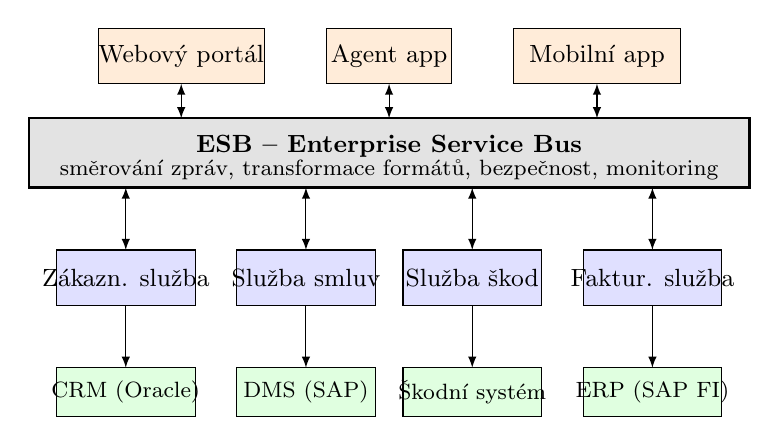
\begin{tikzpicture}[font=\small, scale=0.88, >=latex]
  % ---- Konzumenti (horni vrstva) ----
  \draw[fill=orange!15] (-4.2,4.0) rectangle (-1.8,4.8);
  \node at (-3.0,4.4) {Webový portál};
  \draw[fill=orange!15] (-0.9,4.0) rectangle (0.9,4.8);
  \node at (0,4.4) {Agent app};
  \draw[fill=orange!15] (1.8,4.0) rectangle (4.2,4.8);
  \node at (3.0,4.4) {Mobilní app};

  % ---- ESB (stredni vrstva) ----
  \draw[fill=gray!22, thick] (-5.2,2.5) rectangle (5.2,3.5);
  \node[font=\small\bfseries] at (0,3.1) {ESB -- Enterprise Service Bus};
  \node[font=\footnotesize] at (0,2.75) {směrování zpráv, transformace formátů, bezpečnost, monitoring};

  % ---- Sluzby (dolni vrstva) ----
  \draw[fill=blue!12] (-4.8,0.8) rectangle (-2.8,1.6);
  \node at (-3.8,1.2) {Zákazn. služba};
  \draw[fill=blue!12] (-2.2,0.8) rectangle (-0.2,1.6);
  \node at (-1.2,1.2) {Služba smluv};
  \draw[fill=blue!12] (0.2,0.8) rectangle (2.2,1.6);
  \node at (1.2,1.2) {Služba škod};
  \draw[fill=blue!12] (2.8,0.8) rectangle (4.8,1.6);
  \node at (3.8,1.2) {Faktur. služba};

  % ---- Backendy ----
  \draw[fill=green!12] (-4.8,-0.8) rectangle (-2.8,-0.1);
  \node[font=\footnotesize] at (-3.8,-0.45) {CRM (Oracle)};
  \draw[fill=green!12] (-2.2,-0.8) rectangle (-0.2,-0.1);
  \node[font=\footnotesize] at (-1.2,-0.45) {DMS (SAP)};
  \draw[fill=green!12] (0.2,-0.8) rectangle (2.2,-0.1);
  \node[font=\footnotesize] at (1.2,-0.45) {Škodní systém};
  \draw[fill=green!12] (2.8,-0.8) rectangle (4.8,-0.1);
  \node[font=\footnotesize] at (3.8,-0.45) {ERP (SAP FI)};

  % ---- Sipky konzumenti <-> ESB ----
  \draw[<->] (-3.0,4.0) -- (-3.0,3.5);
  \draw[<->] (0,4.0)    -- (0,3.5);
  \draw[<->] (3.0,4.0)  -- (3.0,3.5);

  % ---- Sipky ESB <-> Sluzby ----
  \draw[<->] (-3.8,2.5) -- (-3.8,1.6);
  \draw[<->] (-1.2,2.5) -- (-1.2,1.6);
  \draw[<->] (1.2,2.5)  -- (1.2,1.6);
  \draw[<->] (3.8,2.5)  -- (3.8,1.6);

  % ---- Sipky Sluzby -> Backendy ----
  \draw[->] (-3.8,0.8) -- (-3.8,-0.1);
  \draw[->] (-1.2,0.8) -- (-1.2,-0.1);
  \draw[->] (1.2,0.8)  -- (1.2,-0.1);
  \draw[->] (3.8,0.8)  -- (3.8,-0.1);
\end{tikzpicture}
\caption{SOA architektura pojišťovny -- ESB integruje heterogenní systémy}
\label{fig:soa}
\end{figure}

\textit{Scénář -- zákazník nahlásí škodu přes webový portál:}
\begin{enumerate}
  \item Webový portál pošle požadavek \textbf{na ESB}: ``Nová škodní událost, zákazník ID 4821''
  \item ESB \textbf{ověří autentizaci} a přesměruje dotaz na \textbf{Zákaznickou službu}:
    ``Existuje zákazník 4821? Má aktivní smlouvu?''
  \item ESB souběžně volá \textbf{Službu smluv}: ``Vrať detail smlouvy zákazníka 4821''
  \item ESB předá data \textbf{Službě škod}: ``Vytvoř novou škodní událost č. SKD-2024-8871''
  \item Služba škod zavolá \textbf{Fakturační službu}: ``Zablokuj pojistné plnění do vyřešení''
  \item ESB vrátí odpověď webovému portálu: ``Škoda přijata, číslo SKD-2024-8871''
\end{enumerate}

Přitom webový portál, mobilní aplikace i agentská aplikace \textbf{všechny sdílí stejné služby}
-- žádný duplicitní kód. Fakturační systém je SAP, CRM je Oracle -- ESB překládá formáty.

\paragraph{SOA vs. Mikroservisy}
\begin{center}
\begin{tabular}{lll}
\toprule
\textbf{Vlastnost} & \textbf{SOA} & \textbf{Mikroservisy} \\
\midrule
Komunikace & ESB (centralizovaná) & REST/gRPC (přímá, decentralizovaná) \\
Granularita & Větší, sdílené služby & Malé, samostatně nasaditelné \\
Technologie & SOAP, WSDL, XML & REST, JSON, gRPC \\
Nasazení & Monolitické bloky & Docker, Kubernetes (kontejnery) \\
Typické použití & Enterprise integrace (ERP, CRM) & Cloud-native aplikace, startupy \\
Příklad & Pojišťovna, banka & Netflix, Amazon, Spotify \\
\bottomrule
\end{tabular}
\end{center}

SOA a mikroservisy sdílejí základní myšlenku (volné propojení, znovupoužitelnost), ale liší se
v granularitě a způsobu komunikace. Mikroservisy jsou v podstatě SOA bez ESB centralizace.

\subsubsection{Přínosy a rizika podnikových IS}

\paragraph{Přínosy}
\begin{itemize}
  \item Zvýšení efektivity procesů a produktivity
  \item Lepší dostupnost a přesnost informací
  \item Podpora strategického rozhodování
  \item Standardizace a optimalizace procesů
  \item Snížení provozních nákladů
\end{itemize}

\paragraph{Rizika implementace}
\begin{itemize}
  \item Překročení rozpočtu a harmonogramu (průměrně 30-40\% IT projektů)
  \item Odpor uživatelů ke změně (change management)
  \item Nekvalitní migrace dat
  \item Nevyhovující přizpůsobení procesů
  \item Závislost na dodavateli (vendor lock-in)
\end{itemize}

\subsubsection{Ekonomické hodnocení IS investic}

\paragraph{Statické metody (bez zohlednění času)}
\begin{itemize}
  \item \textbf{ROI (Return on Investment)} -- $\frac{\text{Čistý zisk}}{\text{Investice}} \times 100\,\%$;
    rychlé porovnání variant
  \item \textbf{TCO (Total Cost of Ownership)} -- celkové náklady vlastnictví: pořizovací náklady + provozní
    náklady za dobu životnosti (licence, HW, podpora, školení, migrace)
  \item \textbf{Payback Period} -- doba, za kterou se investice vrátí z úspor nebo výnosů
\end{itemize}

\paragraph{Dynamické metody (zohledňují časovou hodnotu peněz)}
\begin{itemize}
  \item \textbf{NPV (Net Present Value)} -- čistá současná hodnota; diskontované budoucí toky minus investice;
    NPV $>$ 0 = projekt je výhodný
  \item \textbf{IRR (Internal Rate of Return)} -- vnitřní výnosové procento; diskontní sazba, při které NPV = 0
  \item \textbf{PI (Profitability Index)} -- $\frac{\text{PV budoucích toků}}{\text{Investice}}$; PI $>$ 1 = výhodné
\end{itemize}

\paragraph{ABC (Activity-Based Costing)}
Kalkulace nákladů dle aktivit -- přiřazuje náklady ke konkrétním IT aktivitám a službám;
umožňuje přesněji vyhodnotit nákladovost jednotlivých IS komponent nebo procesů.

\paragraph{Benchmarking IS}
Porovnání výkonnosti IS s odvětvovými standardy nebo konkurencí (Gartner IT benchmarks, ITIL benchmarking).

\begin{profesorbox}[Otázky profesorů k tématu: Podnikové IS]
\textbf{Pour Jan, doc. Ing., CSc.}
\begin{itemize}
  \item Co je ERP a jaké jsou jeho typické moduly?
  \item Jaké jsou 4 etapy implementace podnikového IS?
  \item Jaký je rozdíl mezi CRM a ERP?
\end{itemize}
\textbf{Řepa Václav, prof. Ing., CSc.}
\begin{itemize}
  \item Jaký je rozdíl mezi IASW a TASW? Kdy co použít?
  \item Jaké jsou přínosy a rizika implementace podnikového IS?
\end{itemize}
\textbf{Chudán David, Ing., Ph.D.}
\begin{itemize}
  \item Co je SaaS a jak se liší od IaaS a PaaS?
  \item Co je SOA a jaké jsou jeho výhody?
\end{itemize}
\textbf{Maryška Miloš, doc. Ing., Ph.D.}
\begin{itemize}
  \item Co je MES a jak se liší od ERP?
  \item Jaký je rozdíl mezi Public, Private a Hybrid cloud?
\end{itemize}
\textbf{Sudzina František, Mgr.\ et Mgr.\ Ing., Ph.D.}
\begin{itemize}
  \item Co je SCM a jaké jsou jeho hlavní funkce?
  \item Jaké jsou výhody cloudových IS oproti on-premise řešením?
\end{itemize}
\end{profesorbox}
